% !TEX encoding = UTF-8
% !TEX TS-program = pdflatex
% !TEX root = ../tesi.tex

%TODO cambiare tutti i plugin in sinonimo
%**************************************************************
\chapter{Introduzione}
\label{cap:introduzione}
%**************************************************************

% Introduzione al contesto applicativo.\\

% \noindent Esempio di utilizzo di un termine nel glossario \\
% \gls{api}. \\

% \noindent Esempio di citazione in linea \\
% \cite{site:agile-manifesto}. \\

% \noindent Esempio di citazione nel pie' di pagina \\
% citazione\footcite{womak:lean-thinking} \\

%**************************************************************
\section{Il progetto}   \label{secProgetto}
%Descrizione dell'azienda.
Finantix è un'azienda di informatica che vende un prodotto software principale.
Questo prodotto, per la realizzazione di applicazioni finanziarie, è suddiviso in moduli.
Ognuno di questi moduli prevede una propria documentazione delle API Java (un archivio zip contente documentazione in formato JavaDoc) e la documentazione della API RESTful (un archivio zip contenente documentazione in formato Open API).
Questa documentazione viene manualmente caricata sulla piattaforma Confluence, ove cui è consultata dagli sviluppatori dell'azienda.

%Introduzione all'idea dello stage.
Il plugin Maven nasce dalla necessità di automatizzare la pubblicazione di questa documentazione sulla piattaforma, in modo da semplificare e velocizzare notevolmente questo processo.
Infatti, una volta configurato correttamente il plugin in tutti i progetti relativi ai moduli software, il caricamento della documentazione avviene direttamente durante la build del progetto, senza richiedere ulteriore intervento umano.

    
    Il progetto ha avuto inizio il 10 giugno 2019 ed ha terminato il 2 agosto 2019, per un totale di 320 ore.

    Durante queste 8 settimane, i prodotti attesi erano:
    \begin{enumerate}
        \item \bd{plug-in Maven}: progetto Java il cui risultato è il plugin sopra descritto;
        \item \bd{manuale dell’utilizzatore}: documentazione del plugin Maven che illustra come attivarlo e configurarlo al fine di pubblicare la documentazione generata durante il processo di build sul sistema documentale dell’azienda;
        \item \bd{manuale del programmatore}: descrizione tecnica del plugin Maven, vale a dire, le classi principali dell’implementazione con le relative responsabilità ed il relativo funzionamento.
    \end{enumerate}

    Per raggiungere questo scopo, sono stati fissati alcuni fondamentali obiettivi:
    \begin{itemize}
        \item studiare in maniera autonoma lo strumento Maven per poterne capire appieno l'utilità ed il funzionamento;
        \item comprendere come realizzare un plugin Maven, oggetto centrale del progetto;
        \item comprendere il paradigma RESTful, per poter trasmettere dati al server documentale;
        \item implementare il plugin Maven, una volta raggiunte le competenze sufficienti;
        \item realizzare la documentazione utente, ovvero il manuale dell'utilizzatore sopra citato, per semplificare la comprensione dell'utilizzo del plugin all'utente finale. Non è strettamente necessario all'adempimento del plugin Maven, ma auspicabile;
        \item realizzare la documentazione dello sviluppatore, ovvero il manuale del programmatore sopra citato, per aiutare il programmatore che dovrà fare manutenzione nella cognizione del codice. Anch'esso, come il punto precedente, non è necessario ma auspicabile;
        \item impiegare la tecnologia Jenkins che è usata in azienda per ogni progetto per la continuous integration. Per questo motivo, è possibile farne un minimo utilizzo, ma non è strettamente richiesto.
    \end{itemize}
    
    Tutti gli obiettivi possono essere tracciati da un codice univoco che li identifica. 
    Ognuno di essi ha inoltre una determinata priorità scelta in base all'importanza e necessità di raggiungerli.
    La tabella \ref{obiettiviProgetto} li riassume.
    \begin{table}[H]
		\begin{paddedtablex}[1.7]{\textwidth}{cXc}
			\rowcolor{beautyblue}\textbf{Codice} & \textbf{Descrizione} & \textbf{Priorità} \\
			\toprule
			
            O01 & Acquisizione competenze su Maven & Obbligatorio \\
            O02 & Acquisizione competenze sull’implementazione di plugin Maven & Obbligatorio \\
            O03 & Familiarità con il paradigma RESTFul & Obbligatorio \\
            O04 & Implementazione di un plugin Maven & Obbligatorio \\
            D01 & Documentazione per l’utilizzatore & Desiderabile \\
            D02 & Documentazione per il programmatore & Desiderabile \\
            F01 & Utilizzo di base di Jenkins & Facoltativo \\

			\bottomrule
		\end{paddedtablex}
        \caption{Obiettivi del progetto}
        \label{obiettiviProgetto}
	\end{table}
  
% TODO ampliare 
% Nel piano di lavoro è presente un prospetto che settimana per settimana indica quali attività vengono svolte. L'hai riportato nella tesi? Se l'hai riportato, hai indicato le modifiche all'ordine con cui sono state svolte le attività?




%**************************************************************
\section{Principali problematiche}
Durante il corso dello stage non sono stati riscontrati rilevanti problemi che hanno particolarmente influito sull'attività.
Nonostante ciò, un problema non banale che è stato affrontato riguarda la documentazione di Maven.
Molte pagine relative alla documentazione di plugin Maven infatti, risultano obsolete perché poco aggiornate.
Per far fronte a questo problema, un confronto diretto e costante con gli sviluppatori senior del team DevOps, esperti della tecnologia, è stato il metodo di risoluzione determinante per il proseguimento del progetto.

% \clearpage

%**************************************************************
\section{Strumenti utilizzati}
Gli strumenti adottati per la creazione del plugin Maven sono molteplici.
Alcuni di questi sono abitualmente adoperati da tutti gli sviluppatori dell'azienda, motivo per cui sono stati utilizzati anche per questo progetto, mentre altri sono stati liberamente scelti dalla candidata.
Tra essi, selezionati per i vari motivi sotto elencati, troviamo:
\begin{itemize}
    \item \textbf{GitKraken}: client di Git che presenta un'interfaccia grafica molto intuitiva e interattiva, oltre che semplice da usare;
    % \item \textbf{JUnit}: framework per i test d'unità che si integra facilmente con Eclipse e Maven
    \item \textbf{Visual Studio Code}: editor di codice che supporta molti linguaggi, tra cui JSON e HTML \cite{site:visual-studio-code};
    \item \bd{SequenceDiagram.org}: strumento online che permette la creazione di diagrammi di sequenza in modo semplice e veloce grazie ad una sintassi propria;
    \item \bd{ObjectAid UML Explorer}: estensione di Eclipse che permette la creazione automatica di diagrammi delle classi a partire dal codice Java;
    \item \bd{Meecrowave}: framework, tra i vari consigliat dall'azienda, che permette la creazione di server velocemente \cite{site:meecrowave}.
\end{itemize}

    \subsection{Maven} \label{mavenSection} % TODO rileggere
        
    Maven è un software per la gestione di progetti, basato sul concetto di un ``project object model'' (POM), che gli permette di gestire la build, il report e la documentazione di un progetto Java da un unico pezzo di informazione centrale \cite{site:maven-introduzione}.

    % -------- LIFE CYCLE
    Maven è basato sul concetto di un ciclo di vita della build .
    Ciò significa che il processo per la build e la distribuzione di un particolare artefatto (progetto) è chiaramente definito. 
    Per la persona che realizza un progetto, ciò significa che è solamente necessario imparare un piccolo set di comandi per eseguire la build di un progetto e il POM assicurerà l'ottenimento dei risultati desiderati \cite{site:maven-lifecycle}.
    Ci sono diversi cicli di vita possibili ed ogni ciclo di vita è suddiviso in fasi ben determinate.
    Per esempio, una fase di particolare rilevanza per il progetto del plugin Maven è la fase di \emph{package}, che si occupa di prendere il codice compilato e impacchettarlo nel suo formato distribuibile, come per esempio un JAR. 

    % ------------------

    Ciò che è possibile gestire con questo POM è, per esempio, la lista di dipendeze e i report dei test d'unità, incluso il coverage.
    Il suo aspetto è quello di un file XML che contiene le informazioni riguardanti ul progetto e la sua configurazione, usati da Maven per farne la build.

    % -------- PLUGIN
    \subsubsection{Cos'è un plugin Maven}

    Un plugin è un programma non autonomo che interagisce con un programma per ampliarne o estenderne le funzionalità originarie.
    In questo caso specifico, il programma in questione è Maven.

    Essendo il progetto incentrato sulla realizzazione di un plugin Maven, esso deve avere un \emph{goal}.
    Un \emph{goal} rappresenta un compito specifico (è più fine di una fase) che contribuisce alla gestione del progetto.
    Può essere legato a nessuna, una o più fasi della build.
    Un \emph{goal} non legato ad alcuna fase può essere eseguito al di fuori del ciclo di vita, tramite un'invocazione diretta \cite{site:maven-plugin}.


    Quando viene eseguito un goal, Maven cerca il file ``pom.xml'' (il POM) nella cartella corrente, lo legge, ottiene le informazioni della configurazione e dopo di che esegue il goal.

    Alcune di queste informazioni di configurazione che si possono specificare nel POM possono essere: dipendenze, plugin o goal che possono essere eseguiti, versione e descrizione del progetto, ecc \cite{site:maven-pom}.
    A continuazione, ne viene riportato un esempio.

    % \newpage

    \lstset{frame=tb,
    language=XML,
    aboveskip=3mm,
    belowskip=3mm,
    showstringspaces=false,
    columns=flexible,
    basicstyle={\small\ttfamily},
    numbers=none,
    numberstyle=\tiny\color{gray},
    keywordstyle=\color{black},
    commentstyle=\color{black},
    stringstyle=\color{black},
    breaklines=true,
    breakatwhitespace=true,
    tabsize=3
    }
    \begin{lstlisting} 
    <project>
        <modelVersion>4.0.0</modelVersion>
        <parent>
            <groupId>com.thedigitalstack.maven.plugins</groupId>
            <artifactId>maven-plugins</artifactId>
            <version>1.3.1-SNAPSHOT</version>
        </parent>
        <artifactId>tds-docs-publisher-plugin</artifactId>
        <packaging>maven-plugin</packaging>

        <name>Maven Docs Publisher Plugin</name>
        <description>Maven plug-in to publish generated documentation to 
        Confluence so that official documentation is always up to date with the 
        binary release and easily accessible to authorized users.</description>
        ...
    </project>  
    \end{lstlisting}
    
    % \begin{figure}[H]
    %     \centering
    %     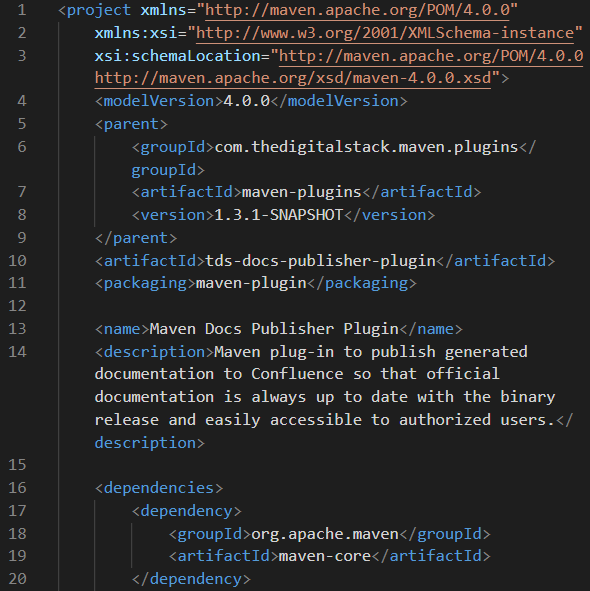
\includegraphics[width=\textwidth]{immagini/screenPOM2.png}\\
    %     \caption{Screenshot di un esempio di POM}
    %     \label{screenPOM}
    % \end{figure}

    % ------------------

    \subsection{Confluence}
    Confluence è un software di collaborazione sviluppato dalla compagnia australiana Atlassian \cite{site:confluence}.
    Esso è il principale sistema documentale dell'azienda, infatti viene usato da ogni dipendente per la consultazione di vario materiale: dalle norme aziendali, alla documentazione del codice.
    Ciò che è più importante, motivo per cui viene utilizzato, è il fatto che permette di raggruppare pagine correlate in uno spazio dedicato accessibile a tutti o a gruppi ristretti di persone.
    
    Recentemente è stato introdotto a Confluence un plugin di terze parti, chiamato \emph{Docs}. 
    Per poter comprendere appieno il progetto del plugin Maven, è prima necessario fare luce su questa estensione di Confluence.

    \subsubsection{Il plugin Docs} \label{pluginDocs}

    \begin{figure}[H]
        \centering
        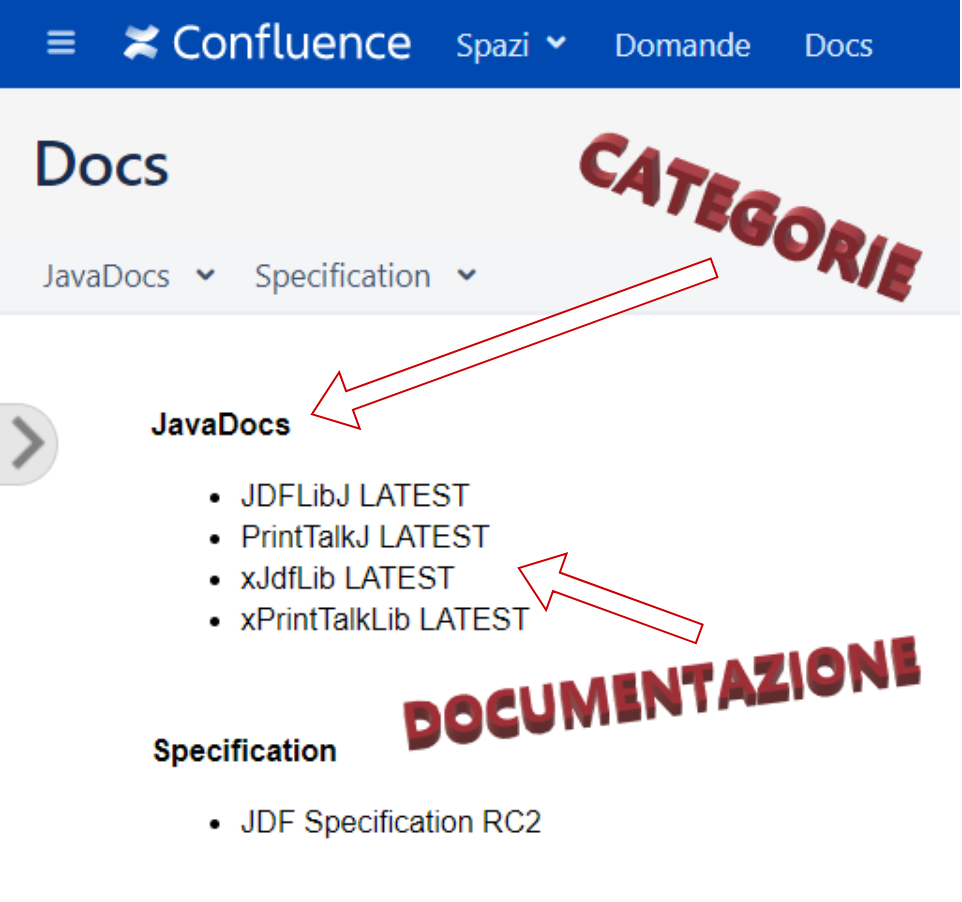
\includegraphics[width=0.56\textwidth]{immagini/docs-conf.png}\\
        \caption{Esempio di Docs Plug-in}
        \label{screenDocs}
    \end{figure}

    Come è possibile vedere dall'immagine \ref{screenDocs}, \emph{Docs} è suddiviso in categorie (in questo caso ``JavaDocs'' e ``Specification'').
    Le categorie presentano un nome, consentono di raggruppare la documentazione e possono essere collegate agli spazi Confluence esistenti, in modo da permettere la visione di questa documentazione solo a determinate persone.
    Ogni categoria quindi contiene al suo interno delle pagine web (chiamate anche \emph{doc}) che includono la documentazione in formato HTML \cite{site:docs-plugin} (come per esempio ``JDF Specification RC2'' per la categoria ``Specification'').

    % \clearpage

    \subsection{Riepilogo degli strumenti}

    La tabella \ref{tabellaStrumenti} riportata in seguito, riassume tutti gli strumenti utilizzati e a quale scopo.

        \begin{table}[H]
            {\def\arraystretch{1.5}
            \begin{tabularx}{\textwidth}{cX}
                \rowcolor{beautyblue}
                \textbf{Strumento} &
                \textbf{Scopo} \\ \hline
                Java & Linguaggio di programmazione \\
                Eclipse & Ambiente di sviluppo \\
                Maven & Build automation per la gestione di progetti \\
                Confluence & Pubblicazione, creazione e consultazione di documentazione \\
                Jira & Issue tracking system \\
                Jenkins & Continuous integration \\
                SonarQube & Analisi statica del codice \\
                Bitbucket e GitKraken & Controllo di versione \\
                JUnit & Test di unità \\
                Visual Studio Code & Editor di codice \\
                SequenceDiagram.org & Creazione dei diagrammi di sequenza \\
                ObjectAid UML Explorer & Creazione dei diagrammi delle classi \\
                Meecrowave & Creazione di server \\
            \end{tabularx}} \\
        \caption{Tecnologie utilizzate durante il progetto e loro scopo.}
        \label{tabellaStrumenti}
        \end{table}

\clearpage

%**************************************************************
\section{Il prodotto ottenuto}

\begin{figure}[H]
    \centering
    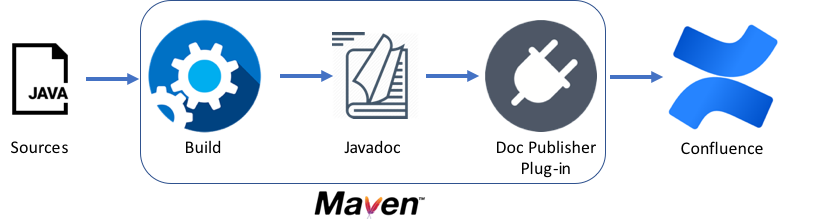
\includegraphics[width=\textwidth]{intro}\\
    \caption{Schema riassuntivo del prodotto}
    \label{screenDocs}
\end{figure}

Il plugin Maven riesce a realizzare il caricamento di documentazione grazie ad un plugin di terze parti su Confluence, chiamato \emph{Docs}, descritto nella sezione \S\ref{pluginDocs}.

Ciò che fa il plugin Maven è caricare su \emph{Docs} in maniera automatica la documentazione nella corretta categoria, realizzando un nuovo \emph{doc} o aggiornandone uno esistente.

Nel caso in cui il titolo fornito per la pagina \emph{doc} non sia presente in \emph{Docs}, verrà creata una nuova pagina, altrimenti il \emph{doc} già esistente con quel nome verrà aggiornato con la documentazione data.

%**************************************************************
\section{Organizzazione del testo}

\begin{description}
    \item[{\hyperref[cap:analisi-requisiti]{Il secondo capitolo}}] comprende l'analisi dettagliata del prodotto, elencandone successivamente i relativi requisiti individuati.

    \item[{\hyperref[cap:progettazione]{Il terzo capitolo}}] spiega la progettazione e la realizzazione del software, descrivendo le tecnologie utilizzate e l'organizzazione del codice tramite diagrammi.

    \item[{\hyperref[cap:testing]{Il quarto capitolo}}] approfondisce come è stata effettuata l'attività di verifica e validazione, soffermandosi in particolare sull'analisi statica del codice e il testing.

    \item[{\hyperref[cap:conclusioni]{Il quinto capitolo}}] corrisponde al capitolo conclusivo. Esso riassume il risultato finale ottenuto e la valutazione critica del prodotto attuata.

\end{description}

Riguardo la stesura del testo, relativamente al documento sono state adottate le seguenti convenzioni:
\begin{itemize}
	% \item gli acronimi, le abbreviazioni e i termini ambigui o di uso non comune menzionati vengono definiti nel glossario, situato alla fine del presente documento;
	% \item per la prima occorrenza dei termini riportati nel glossario viene utilizzata la seguente nomenclatura: \emph{parola}\glsfirstoccur;
	\item i termini in lingua straniera o facenti parti del gergo tecnico sono evidenziati con il carattere \emph{corsivo};
	\item tutti i concetti che possono essere riassunti, vengono raccolti in una tabella o in un elenco puntato;
	\item citazioni e riferimenti, provenienti da siti o libri, vengono accompagnati dal loro numero identificativo tra parentesi quadre, ad esempio \cite{site:junit-annotation}.
\end{itemize}